\documentclass{scrreprt}

\usepackage[colorlinks=true]{hyperref}
\usepackage{graphicx}

\title{Building for the ARM Cortex-M0 with GNU tools}
\author{James Gowans}

\begin{document}

\maketitle
\section*{Licence}
This work is licensed under the Creative Commons Attribution-ShareAlike 3.0 Unported License. To view a copy of this license, visit http://creativecommons.org/licenses/by-sa/3.0/ or send a letter to Creative Commons, 444 Castro Street, Suite 900, Mountain View, California, 94041, USA.

\section*{Preface}
This guide is intended for a range of audiences from those who have never compiled code with GCC before, to those who are experienced with GNU and want to start writing code for ARM.
This guide does not intend to teach you programming, only building and debugging. You should have some familiarity with C and assembly before attempting to develop code.

\tableofcontents

\newpage
\chapter{Toolchain Overview}
\afterpage{
\begin{landscape}
\begin{figure}
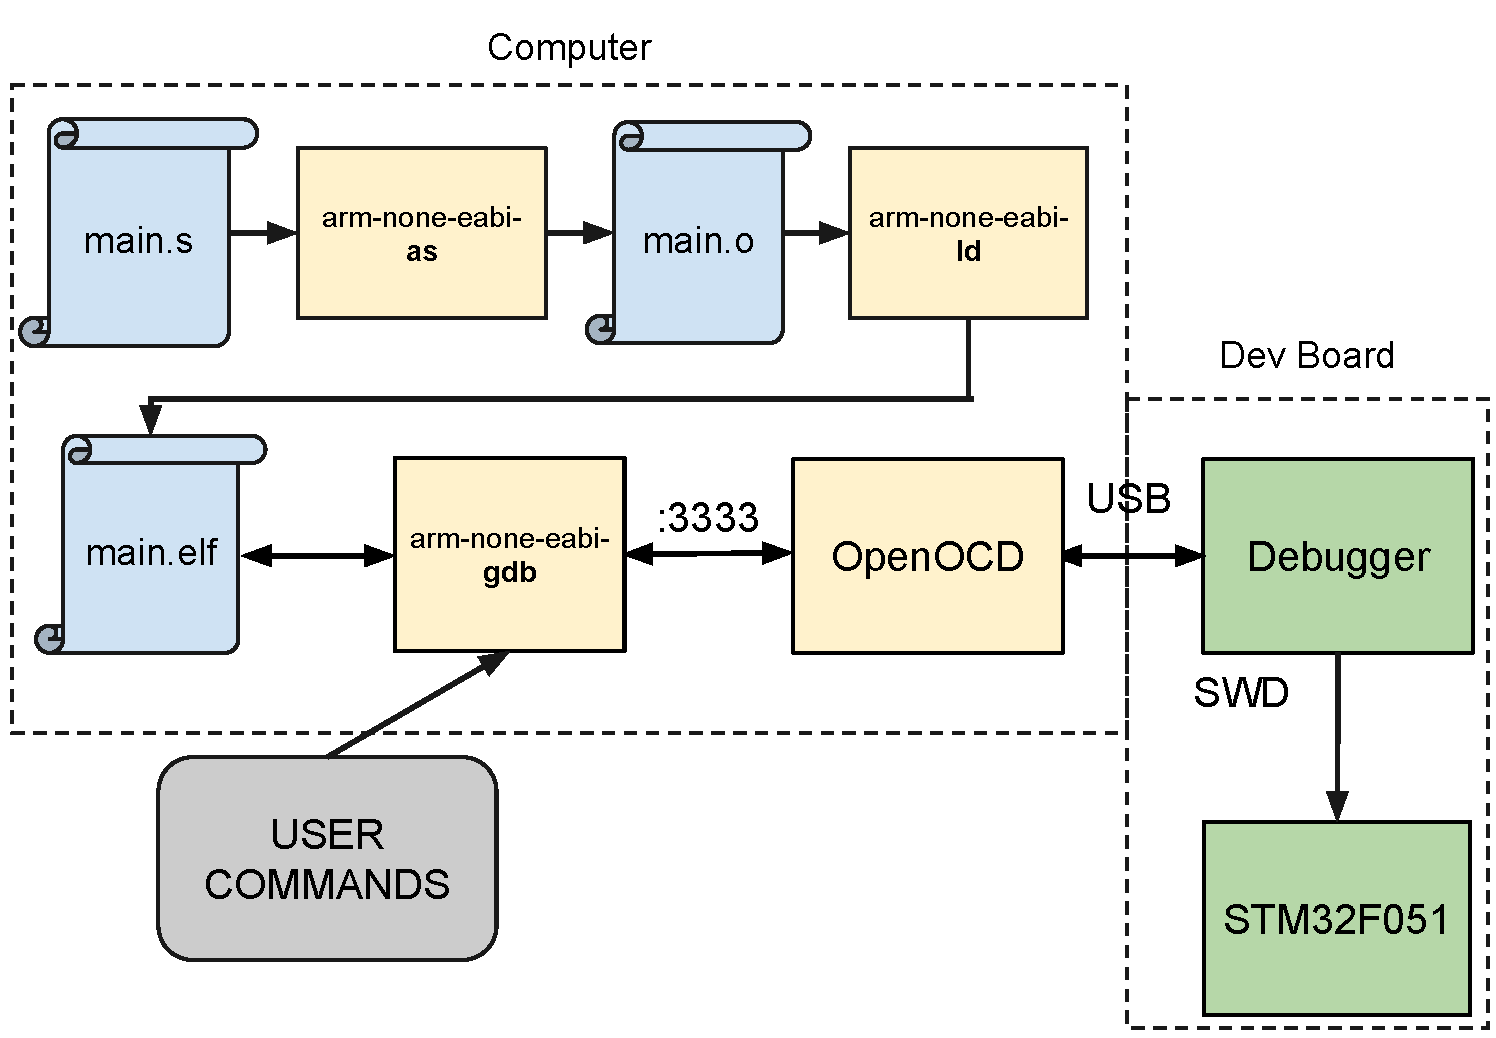
\includegraphics[width=1.4\textwidth]{./img/assembly_to_micro_process.pdf}
\caption{Process which source files takes to be loaded onto micro.}
\label{fig:assembly_to_micro_proc}
\end{figure}
\end{landscape}
}
A toolchain is a collection of software tools that facilitates the process of getting your source code executing on a target platform. This guide will start with the simplest toolchain and introduce more tools and complexity later as required. The simplest set of tools is shown graphically in \autoref{fig:assembly_to_micro_proc} and will now be discussed.

\begin{enumerate}
\item \emph{Text editor:} provides the capability to modify source code files. Typically something like notepad (Windows) or gedit (Linux) will work fine. However, it's recommended for Windows users to install a more customisable editor: Notepad++
\item \emph{Assembler:} converts human-readable assembly code into relocatable (no final address) machine code files. These files are known as object files and are not directly executable. 
\item \emph{Linker:} takes one or more object files and turns them into a single executable which can run directly on the target. The process of linking involves ascertaining the final (absolute) memory address for each section of the executable.
\item \emph{OpenOCD} (On Chip Debugger). This is an interface to the hardware debugger. The hardware debugger microcontroller will typically be connected to the computer via a USB connection. There needs to be a way to send data down the USB cable to the debugger to get it to load code onto the micro or debug running code.
When running in Windows, the ST-Link driver is required. When running in Linux the libusb-1.0 package is required. 
\item \emph{GDB} (GNU debugger) This is a debugger client. It is software which connects to the hardware debugger through the interface and manages what the hardware debugger does by sending it instructions. This can involve sending it executable machine code to load onto the target microcontroller, or causing the target to stop/start/pause execution of the code, or even reading/writing of data in the memory of the target. 
\end{enumerate}

The is a software package called gcc-arm-none-eabi which provides the assembler (arm-none-eabi-as), the linker (arm-none-eabi-ld) as well as the debugger (arm-none-eabi-gdb). 
We will now proceed to review gcc-arm-none-eabi and OpenOCD in some detail.

\section{gcc-arm-none-eabi}
gcc-arm-none-eabi is a fork of the very popular GCC, developed by GNU. This particular fork is maintained by the guys at ARM so it's good software which will probably be around for quite some time. 
The package contains a set of utilities aimed at facilitating the building and debugging of code for ARM processors. 
As discussed earlier, we will be using 3 utilities from this package when building our code, namely \texttt{as}, \texttt{ld} and \texttt{gdb}. 
There are about 25 utilities in total in this package, some more of which we will introduce in the later chapters of this guide. 

A note on the naming convention of \emph{gcc-arm-none-eabi}:
\begin{itemize}
\item \emph{gcc:} This software package is a modification of GCC (GNU Compiler Collection). GNU is a project launched in the late 1980's aiming to promote software freedom. A major part of GNU is the compiler, GCC. 
\item \emph{arm:} This toolchain is designed specifically to operate on code for the ARM family of CPUs.
\item \emph{none:} This refers to the operating system on which the code that is built will run on. ``None'' mean it will not run on an operating system. Rather it will run ``bare-metal'': directly on the hardware. It's worth noting that when we work on a Linux or Windows system and compile code to run on a different platform (in this case: bare-metal), we are doing something known as cross-compiling: compiling code for a different architecture than the compiler is running on.
\item \emph{eabi:} Embedded Application Binary Interface. As far as I can tell, this is some sort of standard or specification which defines how the machine code files which the toolchain produces are structured. By having a standard, it allows our files to be portable and allows files produced by different toolchains to work together.
\end{itemize}

\section{OpenOCD}
This is a program which facilitites communication with hardware over a USB connection. The way it works is that it opens up a port\footnote{If you've never worked with ports before, a port is basically an address which IP traffic can go to. Much like a numbered mailbox, different applications can communicate with each other through ports. One application can place data into the mailbox (send to a port) and another application and receive data from the mailbox (listen on a port). Typically ports are used to communicate between applications on different computers (ie: your computer's browser communicating with a web server on another computer) but nothing stops applications on the same computer also communicating via ports.}
to accept user commands, interprets those commands and passes them to the hardware. It also listens for responses from the hardware and presents that to the user by sending data to whatever application is connected to it. When you launch OpenOCD, you specify two things: the type of hardware you're connecting to (target microcontroller) and the type of hardware debugger which you're connecting to it through. In our case, out target is a STM32F0 family microcontroller and our hardware debugger type is a ST-Link-v2. ST-Link-v2 is the type of firmware which is running on the debugger micro.

Typically, when OpenOCD runs it make a number of ports available to us, each with different purposes. The one which is most important to us is port 3333; the port which deals in GDB traffic. It's designed to have a GDB client connect to it, and it knows how to deal in GDB commands. When we want to use GDB we'll need to connect it to port 3333, which is where OpenOCD is listening for connections and instructions.\\

\subsection{Note on multiple instances of OpenOCD}
Note that only one application can be listening on a port at one time. This means that if another application is listening on port 3333 when OpenOCD launches, it will crash. The further implication of this is that only one instance of OpenOCD can run at a time! If OpenOCD is refusing to run, it may be because you have another instance of it running. Kill all running instances of OpenOCD (or to be really sure: reboot your computer) if OpenOCD won't launch.



\end{document}
